% Monte Carlo Tree Search presentation part

\begin{frame}{Optymalizacja jako ciąg decyzji}
  Budujemy rozwiązanie wykonując ciąg \emph{akcji} prowadzących ze \emph{stanu
  początkowego} do \emph{stanu końcowego}.
  \pause
  \begin{itemize}
    \item \emph{Stan} -- częściowy opis rozwiązania
      \begin{itemize}
        \item początkowy -- częsciowy opis, który ,,pasuje'' do każdego
          rozwiązania dopuszczalnego
        \item końcowy -- reprezentuje jedno rozwiązanie dopuszczalne
      \end{itemize}
      \pause
    \item \emph{Akcja} -- przeprowadza pomiędzy stanami
      \begin{itemize}
        \item najczęściej wiele akcji z danego stanu
        \item problem: którą wybrać?
      \end{itemize}
  \end{itemize}
\end{frame}

\begin{frame}{Stan dla m,s-TSP}
  Ścieżka prosta lub cykl Hamiltona
  \begin{figure}[H]
    \centering
    \begin{tikzpicture}
      [shorten >=1pt,auto,node distance=3cm, thick,main
      node/.style={circle,fill=white!20,draw,font=\sffamily\bfseries}]
      \node[main node] (v0) at (0.1,0.7) {0};
      \node[main node] (v1) at (0.8,2.8) {1};
      \node[main node] (v2) at (2,4.0) {2};
      \node[main node] (v3) at (5,4.8) {3};
      \node[main node] (v4) at (9,5) {4};
      \path (v0) edge node {} (v1);
      \path (v1) edge node {} (v2);
      \path (v2) edge node {} (v3);
      \path (v3) edge node {} (v4);
    \end{tikzpicture}
  \end{figure}
  Stan początkowy -- wybrany wierzchołek, końcowy -- cykl Hamiltona.
\end{frame}

\begin{frame}{Akcja dla m,s-TSP}
  Dołączenie kolejnego wierzchołka (tak aby powstała ścieżka prosta lub cykl Hamiltona)
  \begin{figure}[H]
    \centering
    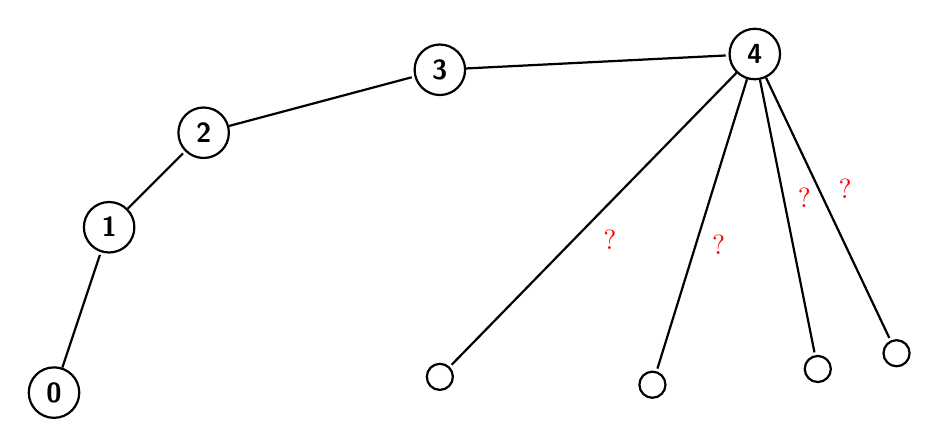
\begin{tikzpicture}
      [shorten >=1pt,auto,node distance=3cm, thick,main
      node/.style={circle,fill=white!20,draw,font=\sffamily\bfseries}]
      \node[main node] (v0) at (0.1,0.7) {0};
      \node[main node] (v1) at (0.8,2.8) {1};
      \node[main node] (v2) at (2,4.0) {2};
      \node[main node] (v3) at (5,4.8) {3};
      \node[main node] (v4) at (9,5) {4};
      \node[main node] (u1) at (10.8,1.2) { };
      \node[main node] (u2) at (9.8,1) { };
      \node[main node] (u3) at (7.7,0.8) { };
      \node[main node] (u4) at (5,0.9) { };
      \path (v0) edge node {} (v1);
      \path (v1) edge node {} (v2);
      \path (v2) edge node {} (v3);
      \path (v3) edge node {} (v4);
      \path (v4) edge node[color=red] {?} (u1);
      \path (v4) edge node[color=red] {?} (u2);
      \path (v4) edge node[color=red] {?} (u3);
      \path (v4) edge node[color=red] {?} (u4);
    \end{tikzpicture}
  \end{figure}
\end{frame}

\begin{frame}{Drzewo decyzyjne}
  Możliwe przebiegi konstrukcji rozwiązania wygodnie reprezentować w formie drzewa...
  \begin{figure}[H]
    \centering
    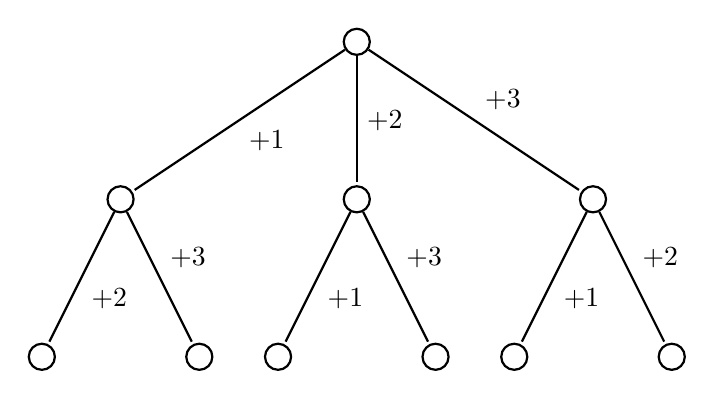
\begin{tikzpicture}
      [shorten >=1pt,auto,node distance=3cm, thick,main
      node/.style={circle,fill=white!20,draw,font=\sffamily\bfseries}]
      \node[main node] (v0) at (6,10) { };
      \node[main node] (v1) at (3,8) { };
      \node[main node] (v2) at (6,8) { };
      \node[main node] (v3) at (9,8) { };
      \node[main node] (v4) at (2,6) { };
      \node[main node] (v5) at (4,6) { };
      \node[main node] (v6) at (5,6) { };
      \node[main node] (v7) at (7,6) { };
      \node[main node] (v8) at (8,6) { };
      \node[main node] (v9) at (10,6) { };
      \path (v0) edge node {+1} (v1);
      \path (v0) edge node {+2} (v2);
      \path (v0) edge node {+3} (v3);
      \path (v1) edge node {+2} (v4);
      \path (v1) edge node {+3} (v5);
      \path (v2) edge node {+1} (v6);
      \path (v2) edge node {+3} (v7);
      \path (v3) edge node {+1} (v8);
      \path (v3) edge node {+2} (v9);
    \end{tikzpicture}
  \end{figure}
  ... którego wygenerowanie leży poza naszym zasięgiem
\end{frame}

\begin{frame}{Monte Carlo Tree Search}
  \begin{block}{Algorytm typu Monte Carlo}
    Algorytm randomizowany, którego czas działania jest deterministyczny, a
    wynik może być niepoprawny z pewnym prawdopodobieństwem.
  \end{block}
  \pause
  \begin{itemize}
    \item przeniesienie jednej z metod implementacji sztucznej inteligencji w
      grach
      \pause
    \item generujemy (mały) spójny podgraf drzewa zawierający jego korzeń
      \pause
    \item decyzje oceniamy na podstawie losowych próbek
  \end{itemize}
\end{frame}

\begin{frame}{MCTS działanie}
  \begin{figure}
    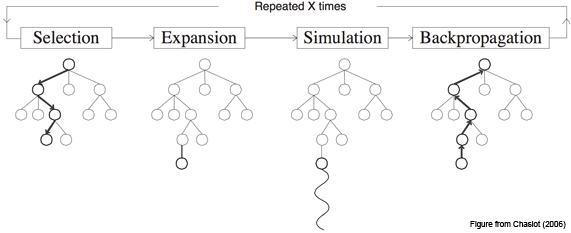
\includegraphics[width=\linewidth]{mcts-algorithm-1a.png}
    \footnote{\url{http://mcts.ai/about/}}
  \end{figure}
\end{frame}

\begin{frame}{MCTS działanie c.d.}
  \begin{itemize}
    \item selekcja (i propagacja wyniku próbki) oraz powiększanie drzewa
      \pause
      \begin{itemize}
        \item eksploracja (słabo poznane decyzje) vs. eksploitacja (obiecujące decyzje)
        \item złożoność pamięciowa
        \item elementy niekoniecznie zależne od problemu
      \end{itemize}
      \pause
    \item próbkowanie
      \begin{itemize}
        \item jedyny element zależny od problemu
      \end{itemize}
  \end{itemize}
\end{frame}

\begin{frame}{Próbkowanie dla m,s-TSP}
  Wykonujemy ciąg losowych decyzji aż osiągamy stan końcowy...
  \begin{figure}[H]
    \centering
    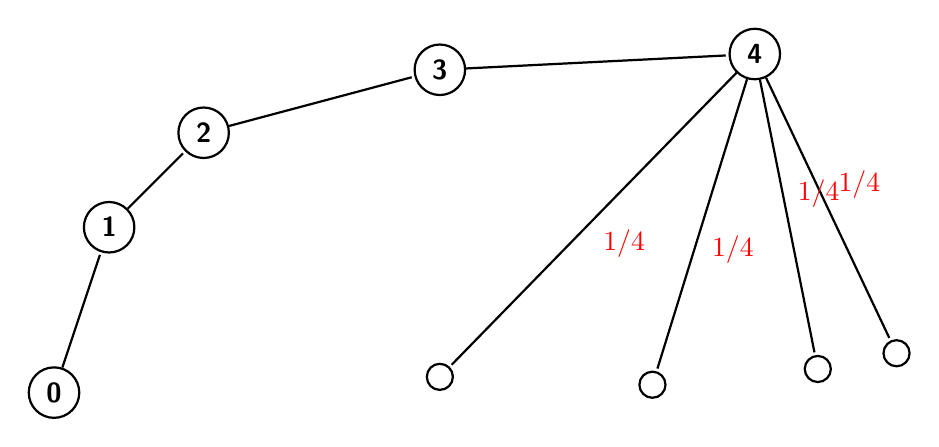
\begin{tikzpicture}
      [shorten >=1pt,auto,node distance=3cm, thick,main
      node/.style={circle,fill=white!20,draw,font=\sffamily\bfseries}]
      \node[main node] (v0) at (0.1,0.7) {0};
      \node[main node] (v1) at (0.8,2.8) {1};
      \node[main node] (v2) at (2,4.0) {2};
      \node[main node] (v3) at (5,4.8) {3};
      \node[main node] (v4) at (9,5) {4};
      \node[main node] (u1) at (10.8,1.2) { };
      \node[main node] (u2) at (9.8,1) { };
      \node[main node] (u3) at (7.7,0.8) { };
      \node[main node] (u4) at (5,0.9) { };
      \path (v0) edge node {} (v1);
      \path (v1) edge node {} (v2);
      \path (v2) edge node {} (v3);
      \path (v3) edge node {} (v4);
      \path (v4) edge node[color=red] {1/4} (u1);
      \path (v4) edge node[color=red] {1/4} (u2);
      \path (v4) edge node[color=red] {1/4} (u3);
      \path (v4) edge node[color=red] {1/4} (u4);
    \end{tikzpicture}
  \end{figure}
  ... w praktyce stosowaliśmy bardziej wyrafinowaną metodę.
\end{frame}

\begin{frame}{MCTS vs. local search dla TSP}
  \begin{figure}
    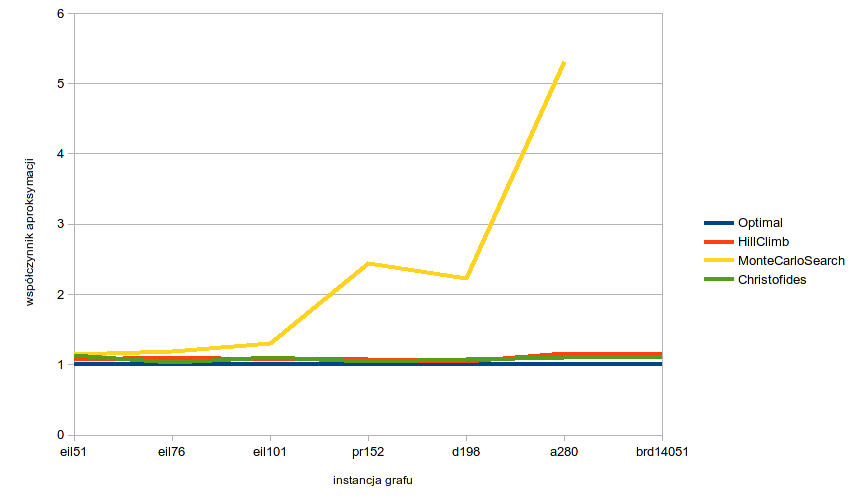
\includegraphics[width=\linewidth]{tsp_comparison.png}
  \end{figure}
\end{frame}
